\subsection{Визуализации представлений}
\label{visual:1}

Продолжая анализ, мы сравниваем векторные представления, которые получаются у нейронных сетей, обученных разными методами (здесь число эпох обучения методов следующее: $t=200$ для SimCLR, $t=200$ для обучения с учителем, $t=30$ для случайной разметки и $t=500$ для случайной разметки с аугментациями). Для этого у нейронных сетей отбрасывается последний линейный слой, после чего обучаются двумерные t-SNE представления (англ. t-distributed stochastic neighbor embedding) \cite{tsne} на выходах предпоследнего слоя для части обучающих объектов. Данные выходы имеют размерность $D=512$. Мы используем случайные 25\% обучающей выборки с сохранением баланса классов (для CIFAR-10 это $0.25 \cdot 50000 = 12500$ объектов).

На рис. \ref{visual:pic:1} изображены обученные t-SNE представления для четырех анализируемых постановок. Метод SimCLR заметно отличается от алгоритмов классификации разметки (истинной или случайной): представления последних образуют четкие кластеры, которые выделяются методом t-SNE. Данные кластеры должны быть линейно разделимыми, чтобы последний линейный слой мог правильно их классифицировать. Разумеется, кластеры согласуются с истинной разметкой только в случае обучения с учителем. При этом добавление аугменаций к обучению со случайной разметкой делает расположение кластеров более плотным.

\begin{figure}[H]
    \centering
    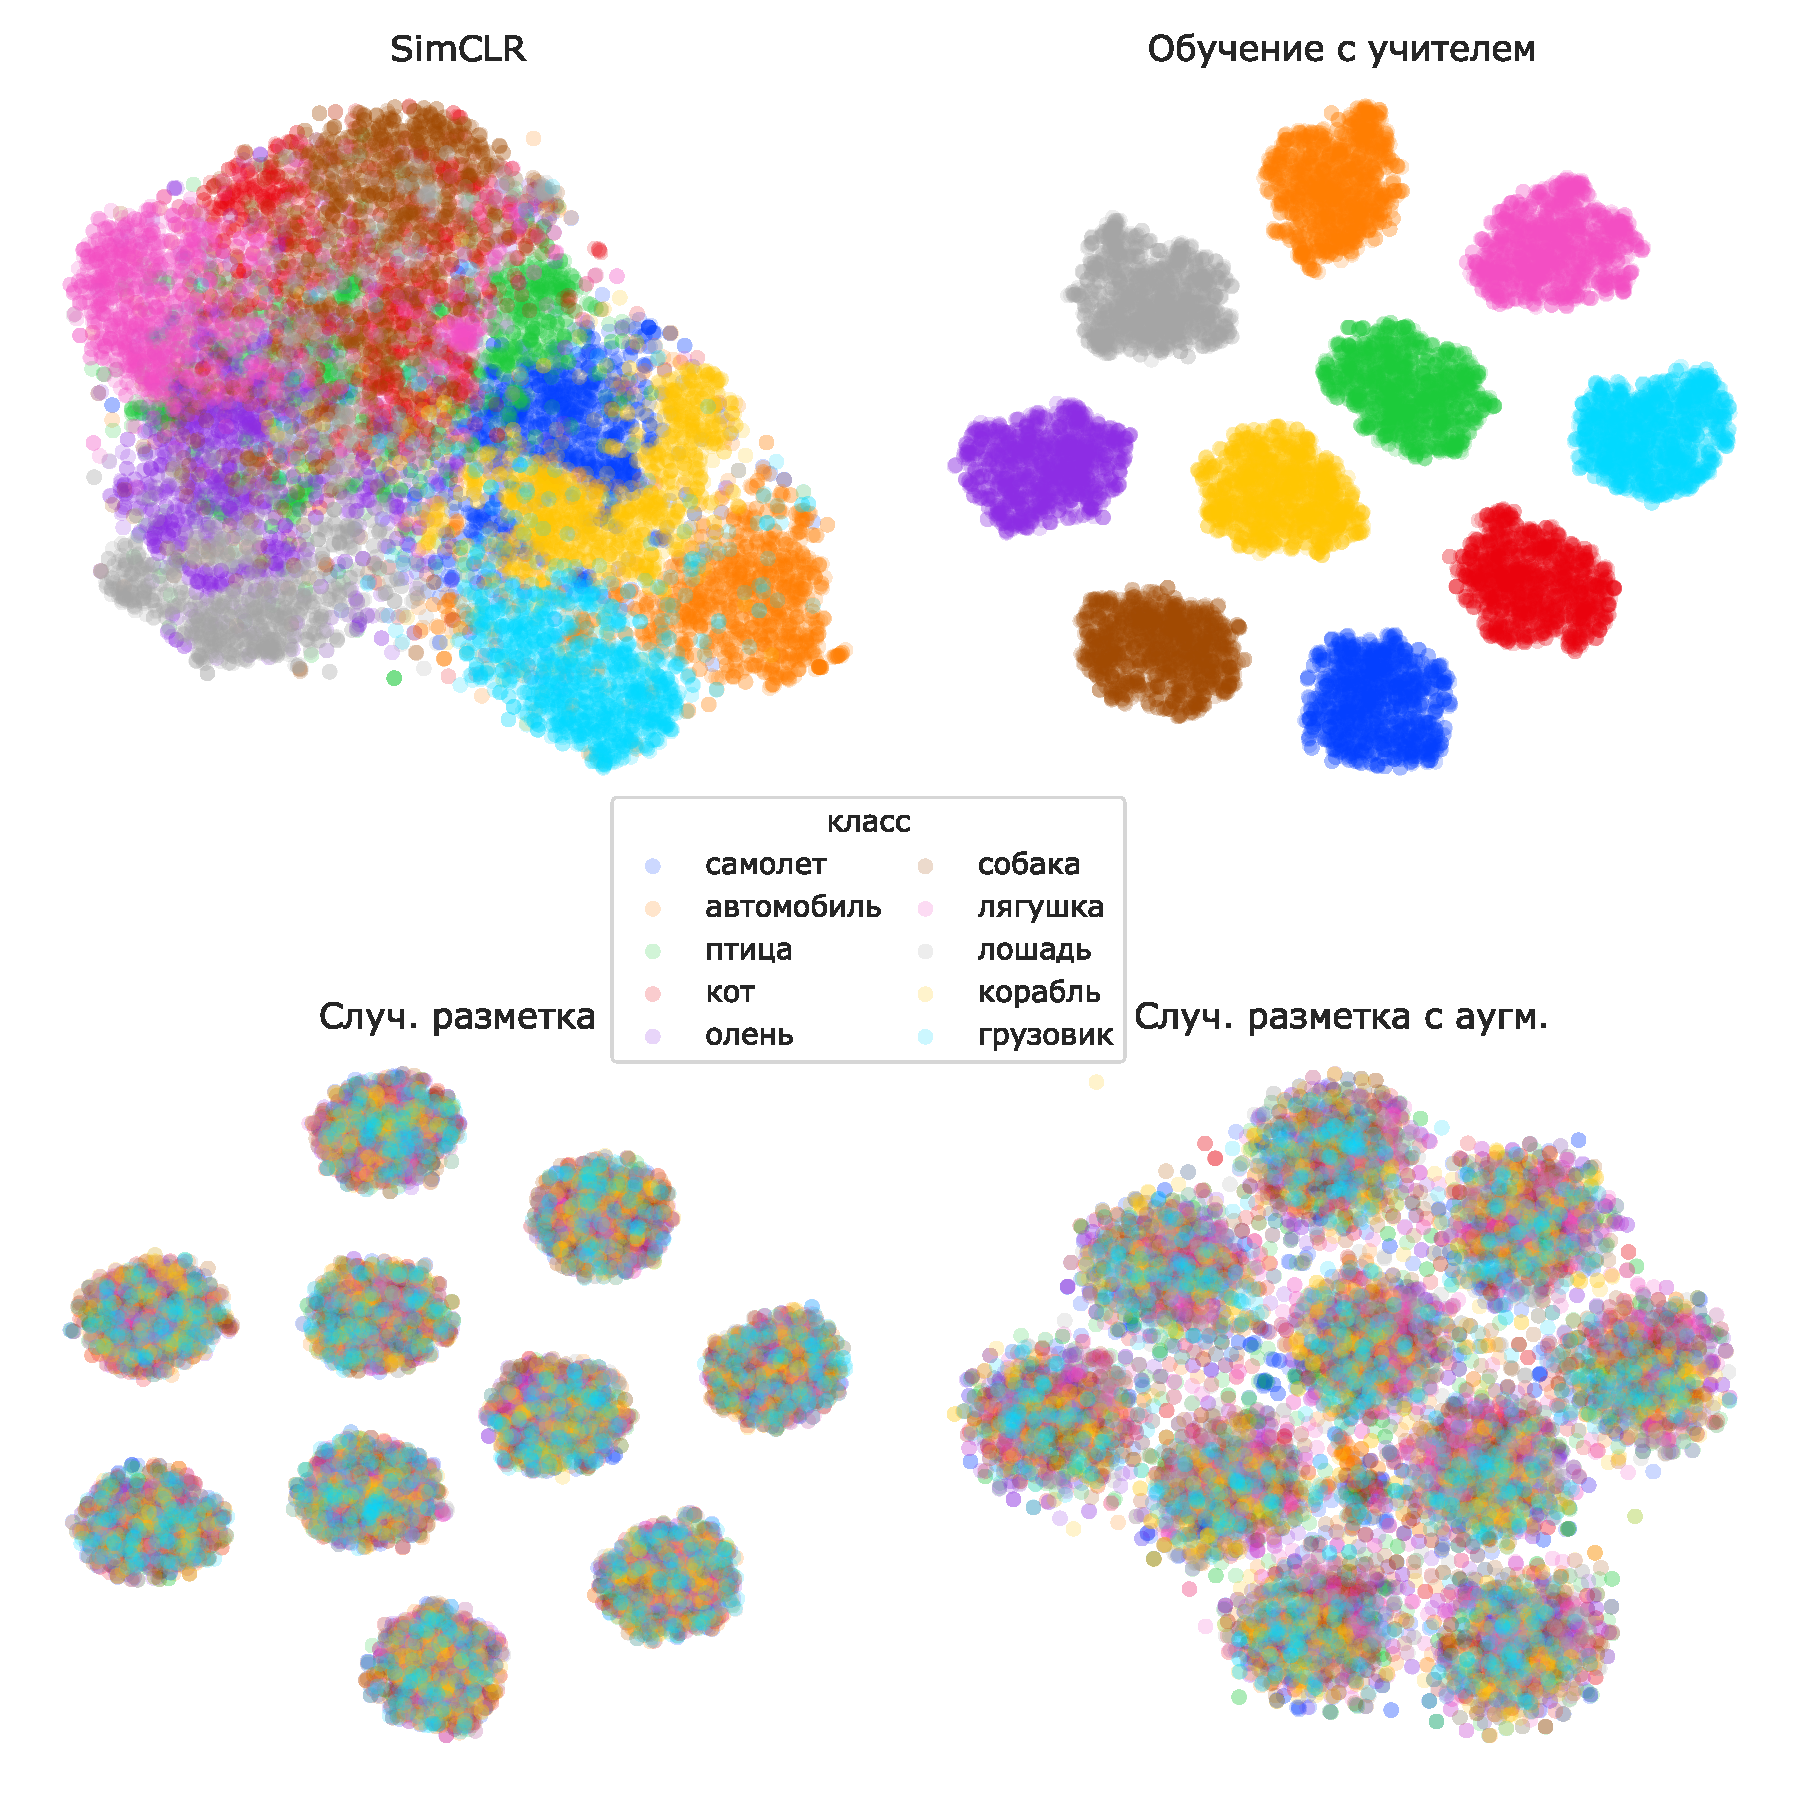
\includegraphics[width=17cm]{images/tsne.pdf}
    \caption{t-SNE представления выходов нейронных сетей, обученных разными методами, для 25\% обучающих объектов. Цветами показана принадлежность обучающих объектов к классам CIFAR-10.}
    \label{visual:pic:1}
\end{figure}{}

Однако наиболее плотное скопление t-SNE представлений наблюдается у алгоритма SimCLR. Это объясняется тем, что нейронная сеть при обучении методом SimCLR не получает сигналов на рассталкивание классов, как происходит при обучении с кросс-энтропийной функцией потерь. Минимизация последней связана не с правильной классификацией обучающих объектов, а с присвоением единичной вероятности истинному классу и нулевой вероятности остальным классам. Поэтому даже если выходы предпоследнего слоя оказываются линейно разделимы, то нейронная сеть продолжает отдалять друг от друга сложившиеся кластеры, повышая верояность истинного класса. В случае метода SimCLR такого эффекта нет, что приводит к более плотному расположению векторных представлений.

Тем не менее, из рис. \ref{visual:pic:1} видно, что t-SNE представления метода SimCLR относительно неплохо согласуются с истинной разметкой по классам. Мы проводим дополнительный эксперимент, сравнивающий взаимное расположение векторных представлений разных классов. Пусть $\{u_k^y\}_{k=1}^{K_y}$ --- это выходы предпоследнего слоя нейронной сети для обучающих объектов класса $y \in \{1, \dots, L\}$, где $L$ --- общее число классов и $u_k^y \in \R^D$. Приблизим распределение $u_k^y$ нормальным $\mathcal{N}_y(\mu_y, \Sigma_y)$ с параметрами:
\begin{equation}
    \mu_y = \frac{1}{K_y} \sum_{k=1}^{K_y} u_k^y \quad\quad \Sigma_y = \frac{1}{K_y - 1} \sum_{k=1}^{K_y} \big(u_k^y - \mu_y\big) \big(u_k^y - \mu_y\big)^T
\end{equation}

\noindent
Мы предлагаем считать KL-дивергенцию между нормальными распределениями, соответствующими разным классам, и сравнивать метод SimCLR и обучение с учителем по данному показателю. Пусть $y, z \in \{1, \dots, L\}$. Тогда KL-дивергенция между распределениями $\mathcal{N}_y(\mu_y, \Sigma_y)$ и $\mathcal{N}_z(\mu_z, \Sigma_z)$ вычисляется по формуле, выведенной в \cite{kl}:
\begin{equation}
\begin{aligned}
    \text{KL}\big(\mathcal{N}_y \big|\big| \mathcal{N}_z\big) = \frac{1}{2} \bigg(\text{Tr}\big(\Sigma_z^{-1} \Sigma_y\big) &+ \big(\mu_z - \mu_y\big)^T \Sigma_z^{-1} \big(\mu_z - \mu_y\big) + \\
    &+ \ln \frac{|\Sigma_z|}{|\Sigma_y|} - D\bigg)
\end{aligned}
\end{equation}

На рис. \ref{visual:pic:2} изображены значения KL-дивергенции, построенные описанным выше способом. Данный эксперимент подтверждает предыдущие выводы: при обучении с учителем векторные представления разных классов оказываются сильно разделены, в то время как SimCLR сохраняет плотную структуру представлений. При этом для метода SimCLR верно, что семантически похожие классы располагаются ближе, чем непохожие: например, дивергенция между классами ''кот'' и ''собака'' заметно меньше, чем между классами ''кот'' и ''автомобиль'' или ''собака'' и ''автомобиль''. Подобное наблюдение можно сделать и для обучения с учителем, но здесь значения KL-дивергенции отличаются в меньшее число раз. Таким образом, векторные представления, которые получаются у метода SimCLR, имеют определенную семантическую структуру, несмотря на то что при обучении не использовалась истинная разметка.

\begin{figure}[H]
    \centering
    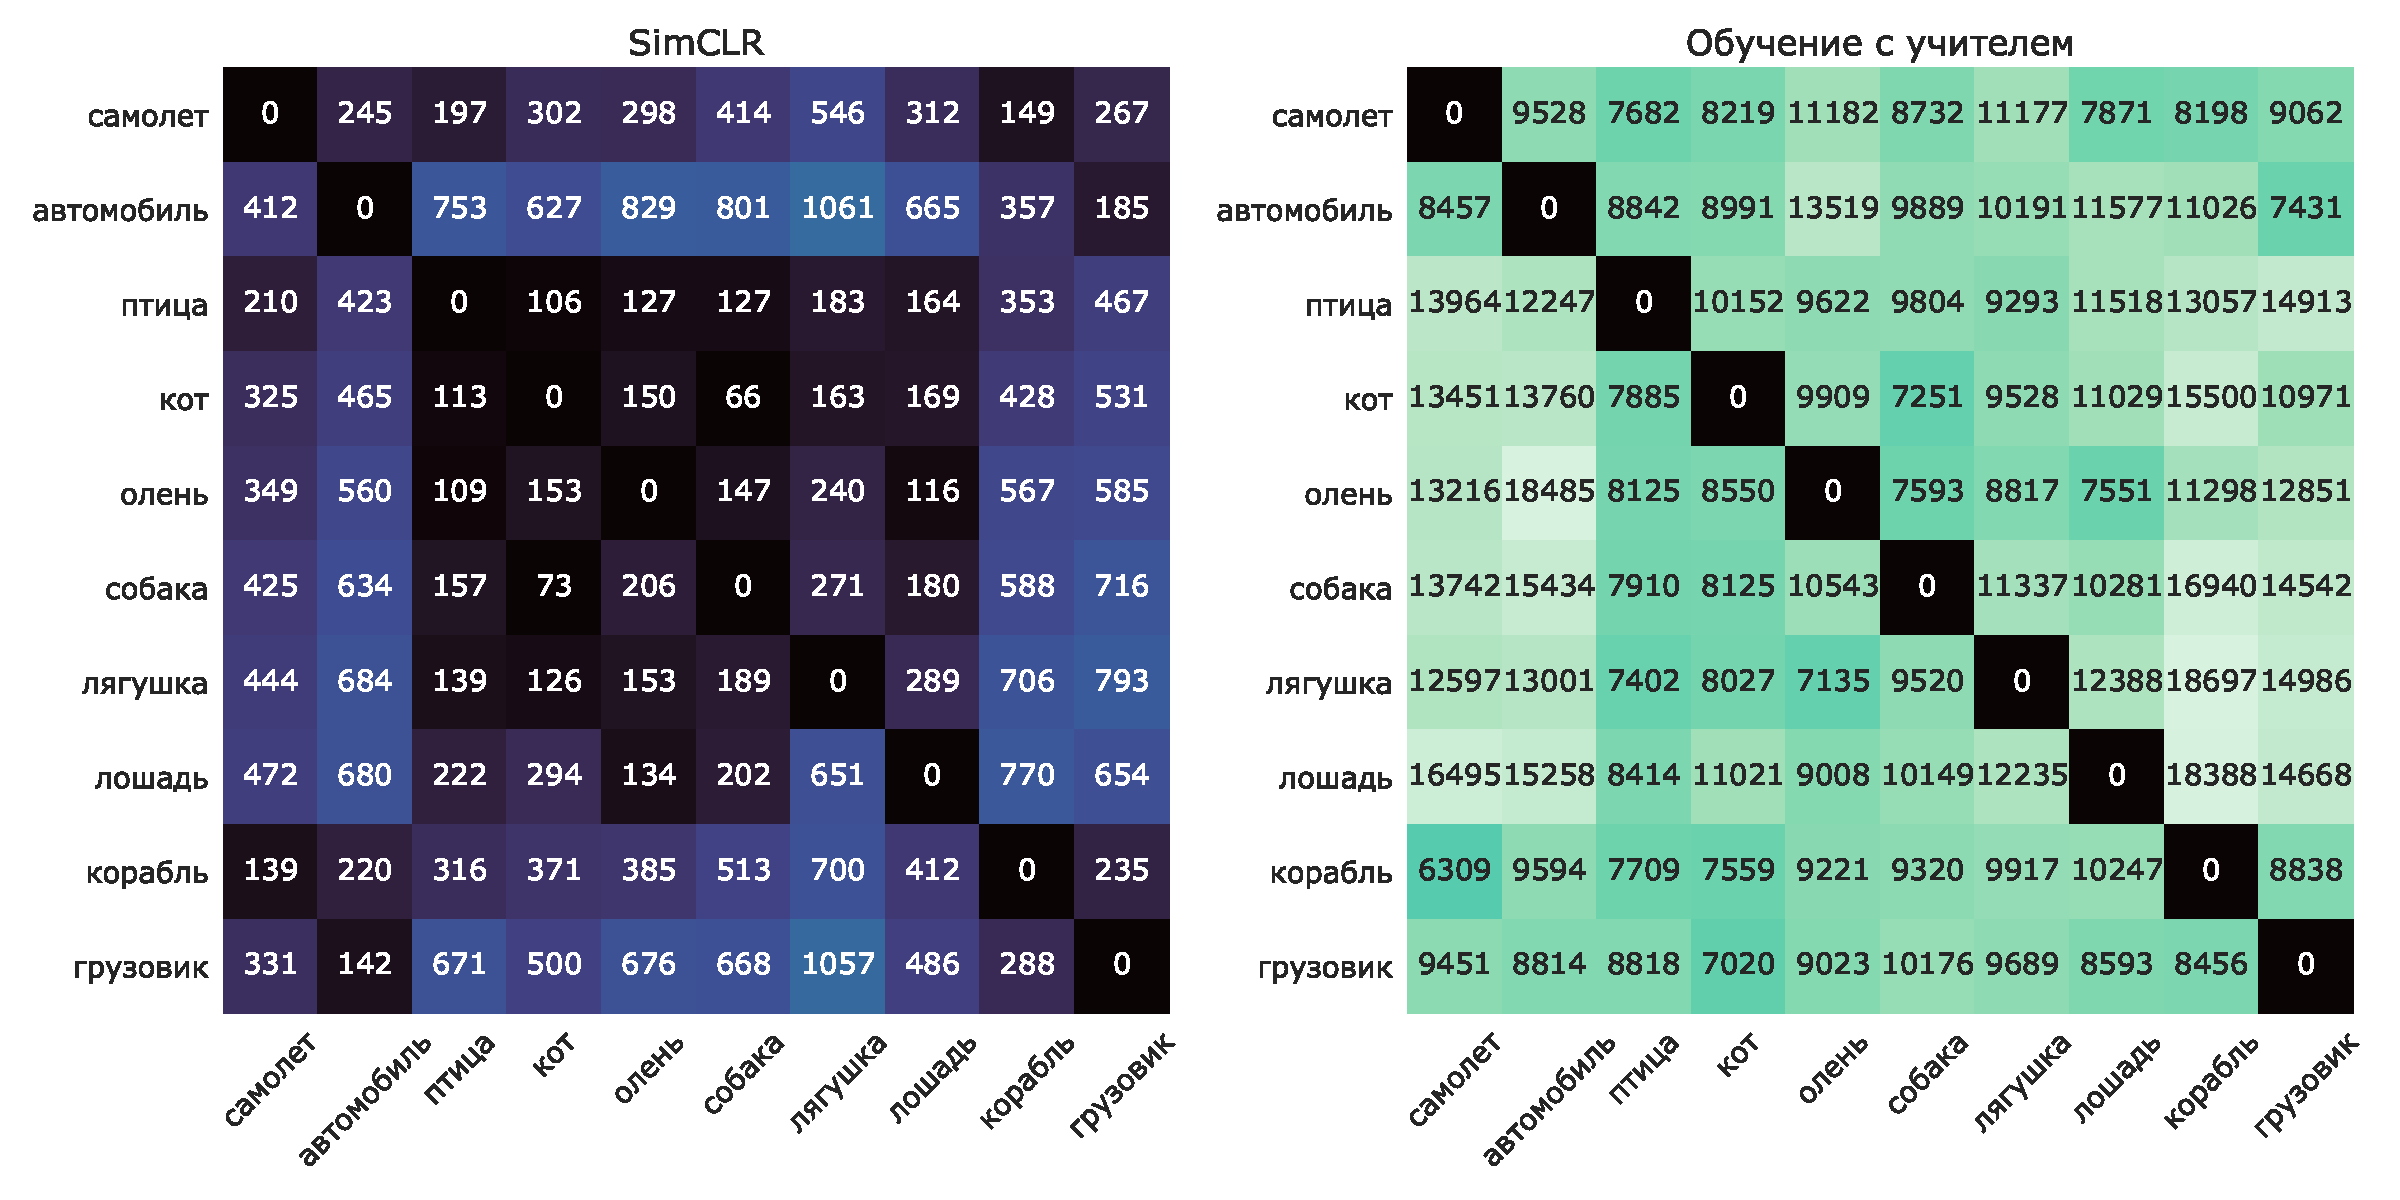
\includegraphics[width=17cm]{images/kl_divergence.pdf}
    \caption{Значения KL-дивергенции между нормальными распределениями, приближающими векторные представления объектов одного класса. Темные цвета соответствуют меньшим значениям дивергенции, светлые --- большим.}
    \label{visual:pic:2}
\end{figure}{}

Мы дополнительно анализируем, являются ли объекты разных классов сложными для выучивания при обучении нейронных сетей. Пусть $\mathcal{D}_y$ означает распределение изображений обучающей выборки, принадлежащих классу $y$. Мы оцениваем величину $\E_{x \sim \mathcal{D}_y} \big[r_t(x)\big]$ методом Монте-Карло:
\begin{equation}
    \E_{x \sim \mathcal{D}_y} \big[r_t(x)\big] \approx \frac{1}{K_y} \sum_{k=1}^{K_y} r_t(x_k^y),
\end{equation}

\noindent
где $\{x_k^y\}_{k=1}^{K_y}$ --- обучающая подвыборка изображений класса $y$. На рис. \ref{visual:pic:3} показана динамика данной величины при обучении методом SimCLR и при обучении с учителем. Из графиков видно, что в задаче классификации выделяются простые (''автомобиль'', ''грузовик'', ''корабль'') и сложные (''кот'', ''птица'', ''собака'') классы, которые выучиваются нейронной сетью, соответственно, быстрее и медленнее. В случае метода SimCLR, напротив, динамика между классами отличается не сильно. В \hyperref[experiments:1]{разделе} 4.2 было показано, что объекты при обучении с учителем значительно отличаются по сложности, и из данного графика следует, что принадлежность изображений разным классам является одной из причин наблюдаемого эффекта.

\begin{figure}[H]
    \centering
    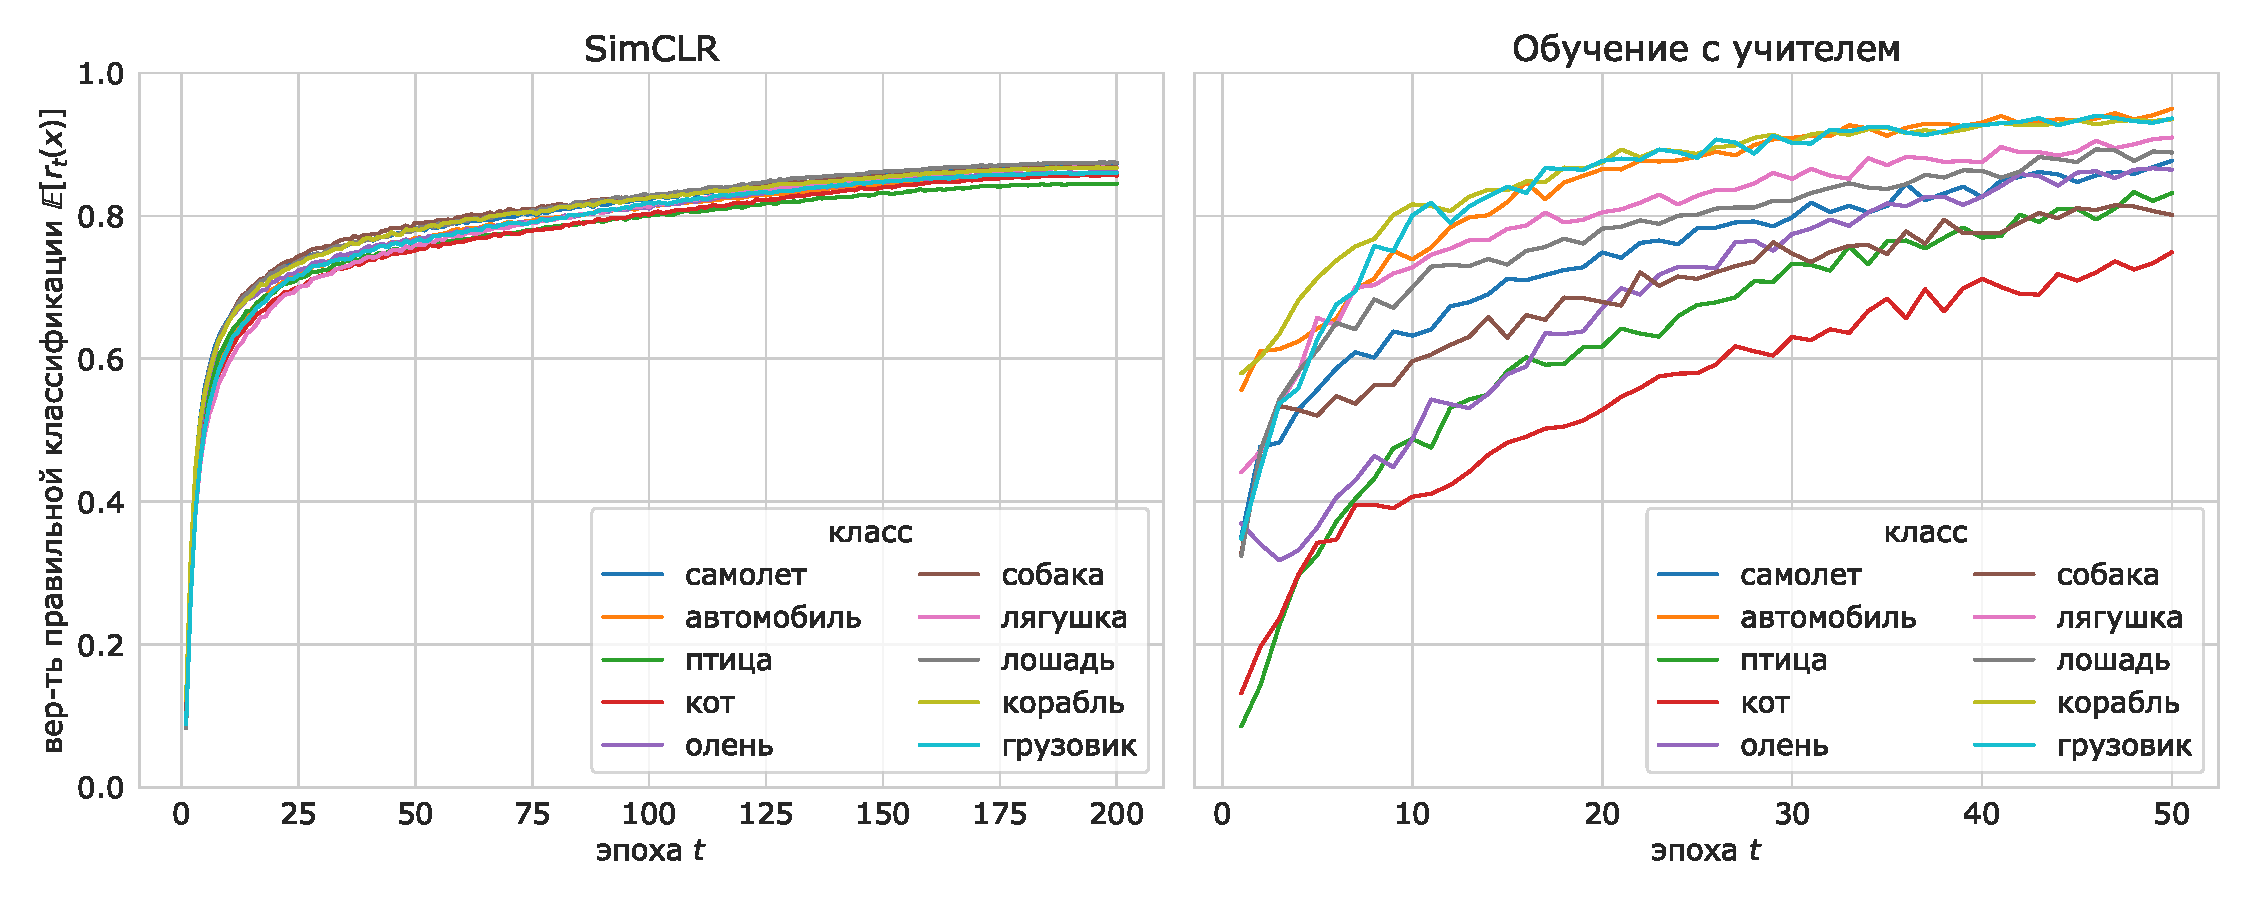
\includegraphics[width=17cm]{images/class_difficulties.pdf}
    \caption{Динамика величины $\E_{x \sim \mathcal{D}_y} \big[r_t(x)\big]$ по эпохам обучения $t$ для разных классов CIFAR-10.}
    \label{visual:pic:3}
\end{figure}{}

\subsection{Визуализации активаций}

В данной работе мы рассматриваем один из самых популярных подходов к визуализации обученных сверточных нейронный сетей --- визуализация рецептивного поля активаций с помощью градиентного подъема в пространстве пикселей \cite{visual}. Рассмотрим некоторую подсеть нейронной сети \linebreak $h: \R^{H_0 \times W_0 \times C} \rightarrow \R$, соответствующую одной активации (одному каналу карты признаков). $H_0 \times W_0$ --- размер рецептивного поля данной активации по отношению ко входу нейронной сети. Пусть тензор $x \in \R^{H_0 \times W_0 \times C}$, максимизурует активацию $h(x)$. Мы будем называть его \textit{псевдоизображением}. Задача оптимизации $h(x)$ по $x$ решается методом градиентного подъема с длиной шага $\eta=1$ и числом итераций $T=1000$. 

\begin{figure}[H]
    \centering
    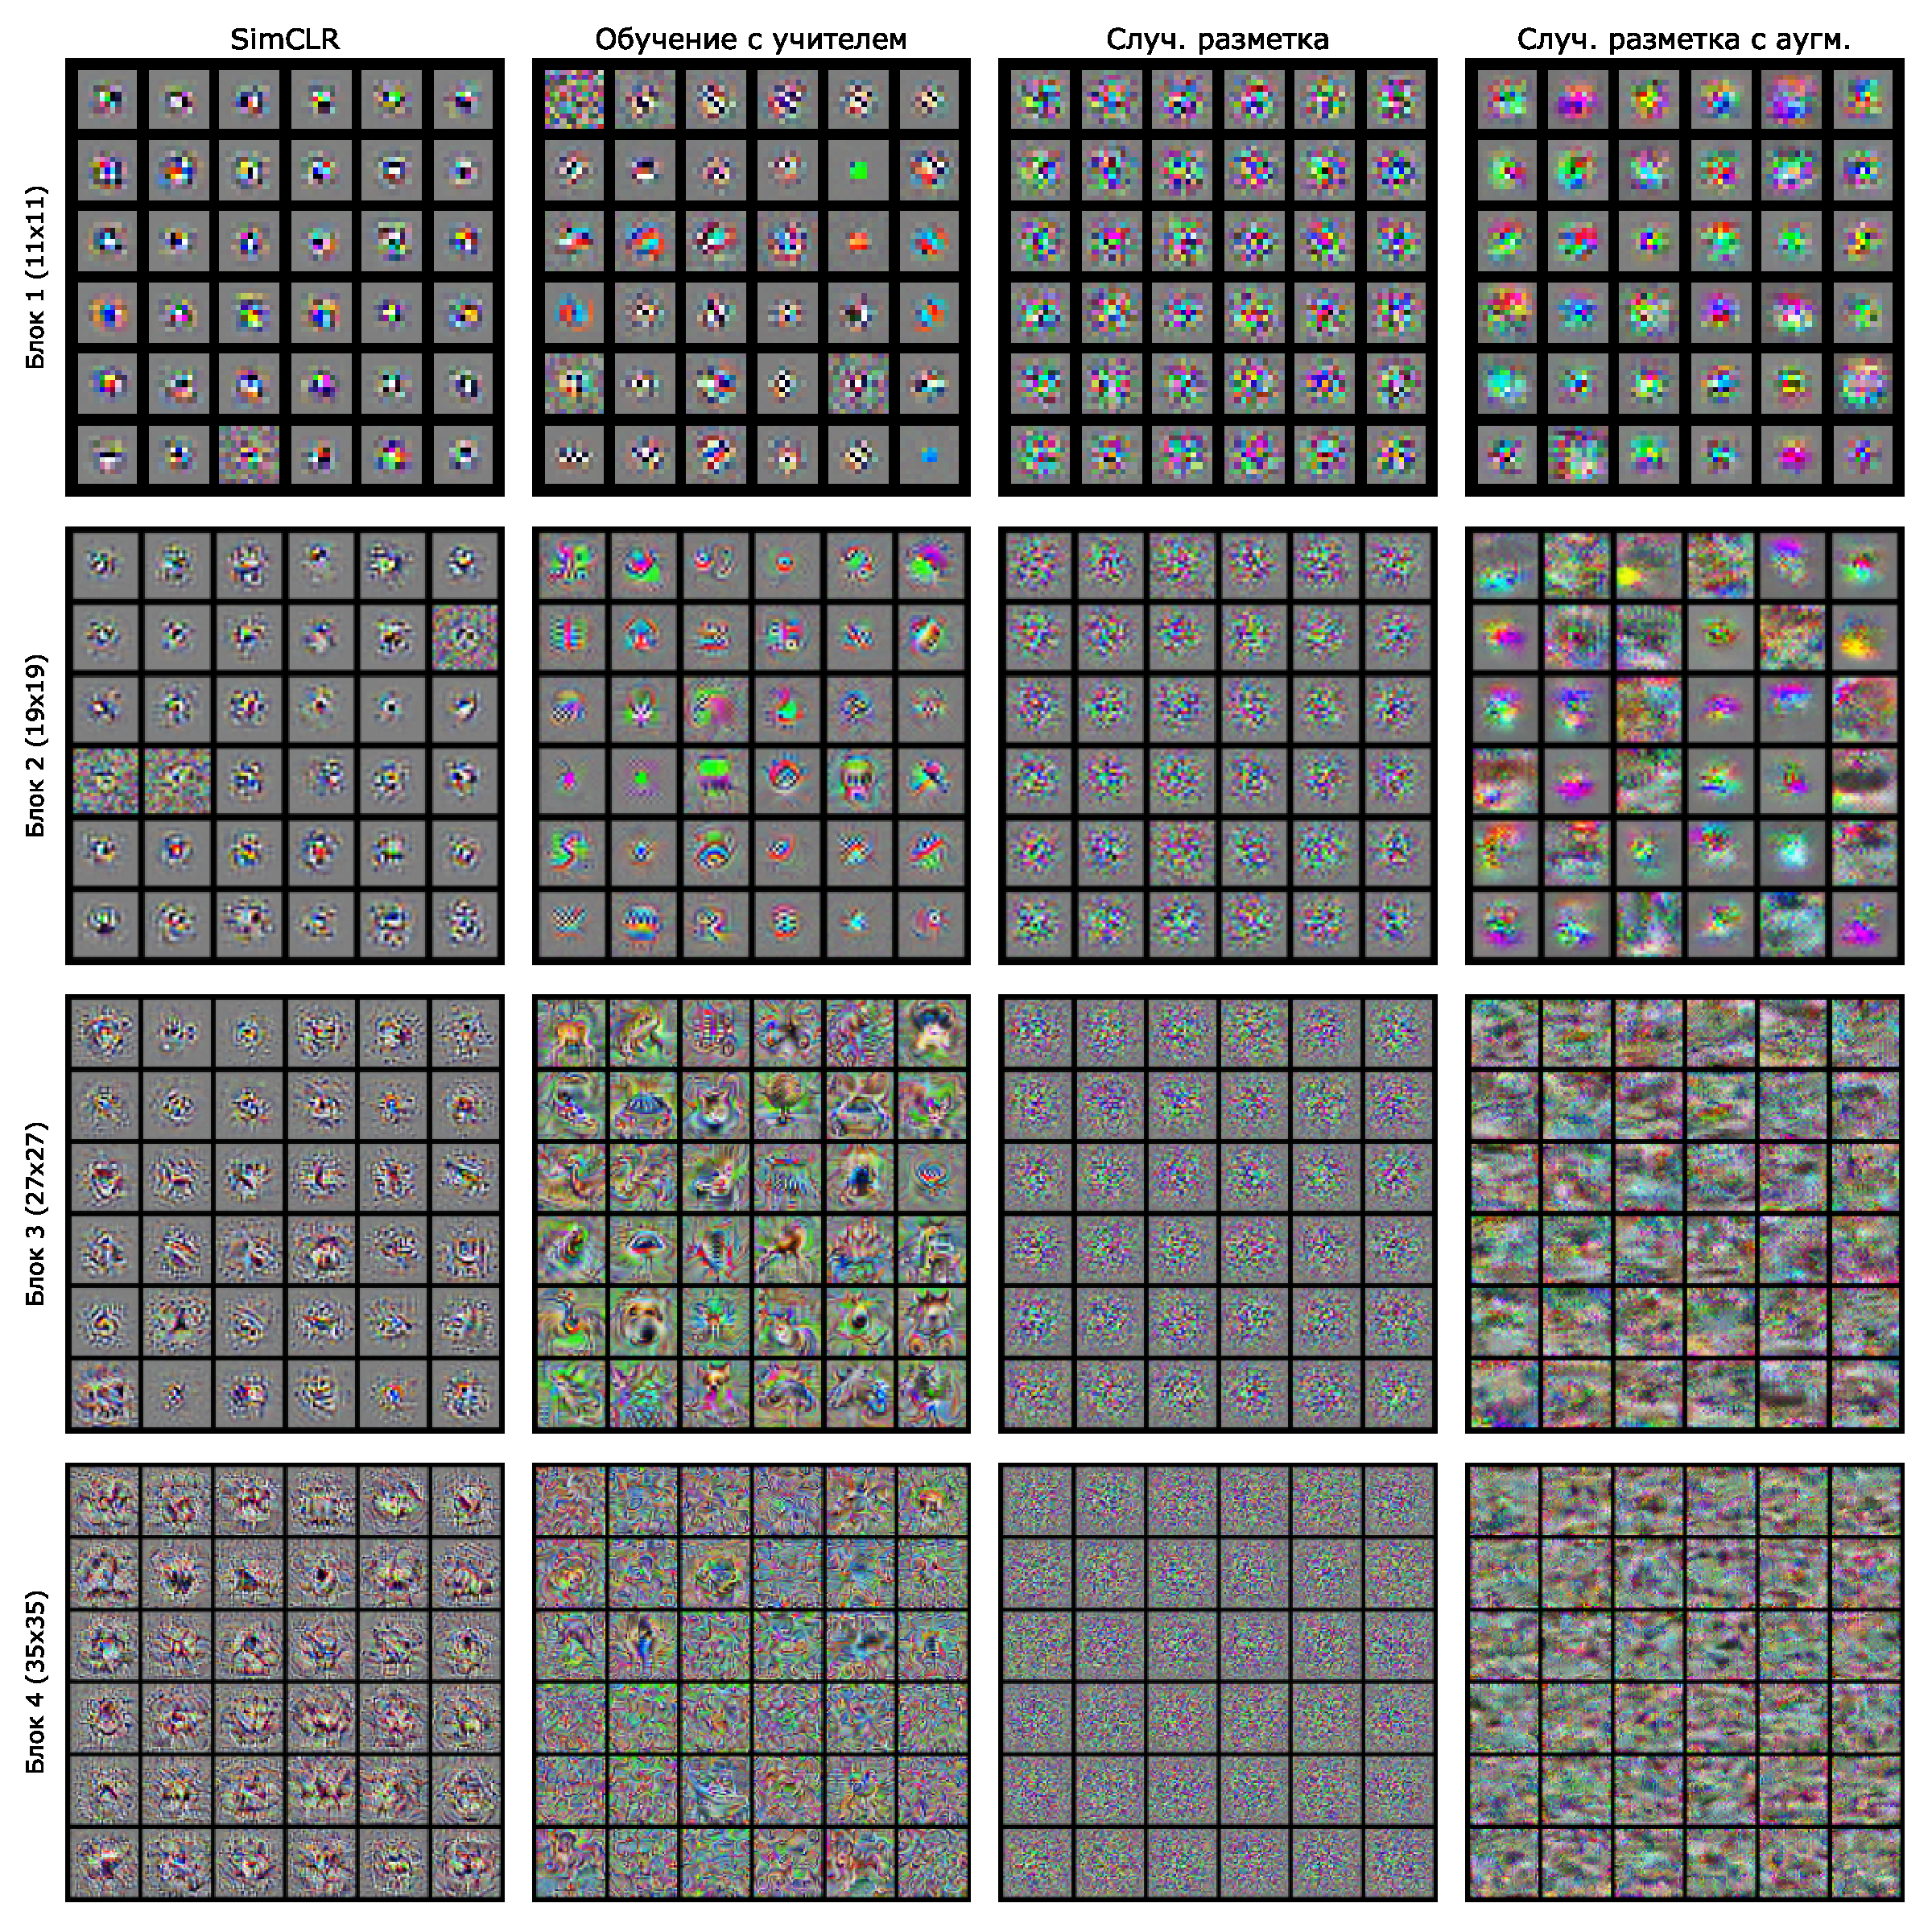
\includegraphics[width=17cm]{images/activations.pdf}
    \caption{Визуализации активаций различных методов. Каждый столбец соответствует своему методу, каждый ряд --- активациям с выхода одного и того же блока архитектуры ResNet-18. В скобках указан размер рецептивного поля активаций $H_0 \times W_0$. Каналы карт признаков для визуализации выбирались случайно, по 36 на каждую пару (метод, блок).}
    \label{visual:pic:4}
\end{figure}{}

Отдельно стоит отметить метод нормализации, который применялся для рисования полученных псевдоизображений. Дело в том, что тензоры, полученные при решении оптимизационной задачи, могут содержать произвольные вещественные числа, в то время как пиксели цветого пространства RGB ограничены отрезком $[0, 1]$. Для каждого псевдоизображения $x$ мы получаем его нормализацию $\hat{x}$ по следующей формуле:
\begin{equation}
\begin{gathered}
    \hat{x} = \sigma \left(\frac{x - \mu_{x}}{s_x}\right)\text{, где} \\
    \mu_x = \frac{1}{H_0 \cdot W_0 \cdot C} \sum_{h, w, c} x_{h, w, c} \quad\quad
    s_x = \sqrt{\frac{1}{H_0 \cdot W_0 \cdot C- 1} \sum_{h, w, c} (x_{h, w, c} - \mu_x)^2}
\end{gathered}
\end{equation}

\noindent
Здесь $\sigma(t)=1/(1+\exp(-t))$ --- логистическая функция, необходимая для отображения значений в отрезок $[0, 1]$.

На рис. \ref{visual:pic:4} показаны визуализации активаций с различных слоев нейронной сети для четырех алгоритмов обучения. Использовался описанный выше метод нормализации псевдоизображений. Сильнее всего выделяются визуализации для обучения со случайной разметкой, которые являются плохо интерпретируемым случайным шумом. Добавление аугментаций в обучение со случайной разметкой значительно меняет активации нейронной сети. Несмотря на то, что на визуализациях не прослеживаются характерные черты изображений CIFAR-10, псевдоизображения куда меньше напоминают шум. Визуализации для обучения с учителем и метода SimCLR похожи друг на друга: простые узоры на ранних слоях (блоки 1--2) переходят в более сложные орнаменты на поздних слоях (блоки 3--4). При этом визуализации метода SimCLR представляются более абстрактными и менее интерпретируемыми. В то же время, среди псевдоизображений обучения с учителем прослеживаются черты, характерные для классов CIFAR-10 (например, силуэт лошадиной \linebreak головы --- блок 3, второй ряд снизу, крайний правый столбец). Последнее наблюдение подтверждает интуицию, что при обучении с учителем нейронная сеть выделяет на обучающих изображениях фрагменты, характерные для классов разметки, и выдает предсказания, основываясь на соответствии входного изображения выделенным фрагментам.
